\section{Results}\label{Sec: Results}
In this section, we present the results of the experiments conducted. The results are in the form of tables and graphs.
The details of the graphs used in the experiments are presented in Table \ref{tab:graph_details}. 
The table \tableref{\ref{tab:ti}} presents the timings for the experiments conducted on the graphs. 
The timings are presented in seconds. 
The timings are compared with the standard static algorithm and the dynamically maintained parallel algorithm. 
The timings are presented for different percentages of updates w.r.t. edges.

The machine specifications are retrieved using the \texttt{lscpu} command. The machine specifications are as follows:
\begin{description}[font=\sffamily\bfseries\small,itemsep=0pt,parsep=0pt]
    \item[Architecture:] x86\_64
    \item[CPU op-mode(s):] 32-bit, 64-bit
    \item[Byte Order:] Little Endian
    \item[CPU(s):] 80
    \item[On-line CPU(s) list:] 0-79
    \item[Thread(s) per core:] 2
    \item[Core(s) per socket:] 20
    \item[Socket(s):] 2
    \item[NUMA node(s):] 2
    \item[Vendor ID:] GenuineIntel
    \item[CPU family:] 6
    \item[Model:] 85
    \item[Model name:] Intel(R) Xeon(R) Gold 6248 CPU @ 2.50GHz
    \item[Stepping:] 7
    \item[CPU MHz:] 1000.061
    \item[CPU max MHz:] 3900.0000
    \item[CPU min MHz:] 1000.0000
    \item[BogoMIPS:] 5000.00
    \item[Virtualization:] VT-x
    \item[L1d cache:] 32K
    \item[L1i cache:] 32K
    \item[L2 cache:] 1024K
    \item[L3 cache:] 28160K
    \item[NUMA node0 CPU(s):] 0-19,40-59
    \item[NUMA node1 CPU(s):] 20-39,60-79
\end{description}

The software specifications are retrieved using the \texttt{gcc --version}, \texttt{mpirun --version}, \texttt{boost --version}, and \texttt{cmake --version} commands.
The kernel and OS specifications, are retrieved using the \texttt{hostnamectl} command. The above specifications are as follows:
\begin{description}[font=\sffamily\bfseries\small,itemsep=0pt,parsep=0pt]
    \item[Operating System:] Red Hat Enterprise Linux Server 7.6 (Maipo)
    \item[Kernel:] 3.10.0-957.el7.x86\_64
    \item[Compiler:] gcc version 9.2.0
    \item[OpenMPI:] 3.1
    \item[Boost:] 1.84.0
    \item[CMake:] 2.8.12.2
\end{description}

\begin{table}[H]
    \centering
    \caption{Graph Details \cite[SNAP Datasets]{snapnets}}
    \begin{tabular}{|c|c|c|}
        \hline
        \textbf{Graph} & \textbf{Number of Vertices} & \textbf{Number of Edges} \\
        \hline
        \texttt{Slashdot0902} & 82168 & 948464 \\
        \texttt{Wiki-Vote} & 7115 & 103689 \\
        \texttt{web-BerkStan} & 685230 & 7600595 \\
        \texttt{web-Google} & 875713 & 5105039 \\
        \texttt{Amazon0302} & 262111 & 1234877 \\
        \texttt{WikiTalk} & 2394385 & 5021410 \\
        \texttt{soc-pokec-relationships} & 1,632,803 & 30,622,564 \\
        \hline
    \end{tabular}
    \label{tab:graph_details}
\end{table}

The each graph, the algorithm was tested by increasing the total number of updates w.r.t. the percentage of edges present in the graph. 
The $0$ percent edge updates, indicates the time taken to initialization the SCC-tree for the maintaince process. 
The subsequent tests conducted, reveal the time taken to update the SCC-tree for the given percentage of updates. 
All the testing was conducted on the same machine, with \texttt{-np} parameter set to $64$ for the \texttt{mpirun} command.


\begin{table}[H]
    \centering
    \caption{Timings for Graphs in \tableref{\ref{tab:graph_details}} }
    \label{tab:ti}
\parbox{0.45\linewidth}{
    \centering
    \caption{\texttt{Amazon0302}}
    \label{tab:Amazon0302}
    \begin{tabular}{|c|c|c|}
        \hline
        \textbf{Update(\%)} & \multicolumn{2}{c|}{\textbf{Timings}} \\
        \hline
        w.r.t. edges & Static &  Dynamic \\
        \hline
        0 & 2.69061 & 9.04671 \\
        1.0 & 2.69061 & 2.09399 \\
        5.0 & 3.01042 & 2.24362 \\
        10.0 & 3.09495 & 2.34654 \\
        20.0 & 3.29579 & 2.6431 \\
        30.0 & 3.40107 & 2.83777 \\
        50.0 & 3.54919 & 3.25233 \\
        \hline
    \end{tabular}
}
\hfill
\parbox{0.45\linewidth}{
    \centering
    \caption{\texttt{Slashdot0902}}
    \label{tab:Slashdot0902}
    \begin{tabular}{|c|c|c|}
        \hline
        \textbf{Update(\%)} & \multicolumn{2}{c|}{\textbf{Timings}} \\
        \hline
        w.r.t. edges & Static &  Dynamic \\
        \hline
        0 & 1.1383 & 5.30846 \\
        1.0 & 1.1383 & 0.509686 \\
        5.0 & 1.17131 & 0.64476 \\
        10.0 & 1.19611 & 0.761259 \\
        20.0 & 1.25575 & 1.04112 \\
        30.0 & 1.4406 & 1.24635 \\
        50.0 & 1.30949 & 1.67949 \\
        \hline
    \end{tabular}
}
\hfill
\parbox{0.45\linewidth}{
    \vspace{1.5em}
    \centering
    \caption{\texttt{Wiki-Vote}}
    \label{tab:Wiki-Vote}
    \begin{tabular}{|c|c|c|}
        \hline
        \textbf{Update(\%)} & \multicolumn{2}{c|}{\textbf{Timings}} \\
        \hline
        w.r.t. edges & Static &  Dynamic \\
        \hline
        0 & 0.102256 & 0.435191 \\
        1.0 & 0.102256 & 0.0353187 \\
        5.0 & 0.108545 & 0.042797 \\
        10.0 & 0.0966422 & 0.0540102 \\
        20.0 & 0.101367 & 0.0726061 \\
        30.0 & 0.0961294 & 0.0943561 \\
        50.0 & 0.118703 & 0.136274 \\
        \hline
    \end{tabular}
}
\hfill
\parbox{0.45\linewidth}{
    \vspace{1.5em}
    \centering
    \caption{\texttt{WikiTalk}}
    \label{tab:WikiTalk}
    \begin{tabular}{|c|c|c|}
        \hline
        \textbf{Update(\%)} & \multicolumn{2}{c|}{\textbf{Timings}} \\
        \hline
        w.r.t. edges & Static &  Dynamic \\
        \hline
        0 & 20.7767 & 37.7838 \\
        1.0 & 20.7767 & 15.4092 \\
        5.0 & 22.2939 & 17.7078 \\
        10.0 & 22.7917 & 18.5541 \\
        20.0 & 23.2082 & 19.1667 \\
        30.0 & 23.4775 & 20.6392 \\
        50.0 & 24.4343 & 23.8523 \\
        \hline
    \end{tabular}
}
\hfill
\parbox{0.45\linewidth}{
    \vspace{1.5em}
    \centering
    \caption{\texttt{web-BerkStan}}
    \label{tab:web-BerkStan}
    \begin{tabular}{|c|c|c|}
        \hline
        \textbf{Update(\%)} & \multicolumn{2}{c|}{\textbf{Timings}} \\
        \hline
        w.r.t. edges & Static &  Dynamic \\
        \hline
        0 & 8.28039 & 39.5969 \\
        1.0 & 8.28039 & 4.10159 \\
        5.0 & 9.12419 & 8.08547 \\
        10.0 & 9.88219 & 10.96283 \\
        20.0 & 11.0039 & 16.96717 \\
        30.0 & 11.4561 & 17.9223 \\
        50.0 & 13.0278 & 18.2617 \\
        \hline
    \end{tabular}
}
\hfill
\parbox{0.45\linewidth}{
    \vspace{1.5em}
    \centering
    \caption{\texttt{web-Google}}
    \label{tab:web-Google}
    \begin{tabular}{|c|c|c|}
        \hline
        \textbf{Update(\%)} & \multicolumn{2}{c|}{\textbf{Timings}} \\
        \hline
        w.r.t. edges & Static &  Dynamic \\
        \hline
        0 & 13.6496 & 42.7283 \\
        1.0 & 13.6496 & 6.87915 \\
        5.0 & 14.4792 & 9.60964 \\
        10.0 & 14.9307 & 10.43506 \\
        20.0 & 15.4813 & 15.0343 \\
        30.0 & 15.8665 & 16.96263 \\
        50.0 & 16.8315 & 23.3846 \\
        \hline
    \end{tabular}
}
\hfill
\parbox{0.45\linewidth}{
    \vspace{1.5em}
    \centering
    \caption{\texttt{soc-pokec-relationships}}
    \label{tab:soc-pokec-relationships}
    \begin{tabular}{|c|c|c|}
        \hline
        \textbf{Update(\%)} & \multicolumn{2}{c|}{\textbf{Timings}} \\
        \hline
        w.r.t. edges & Static &  Dynamic \\
        \hline
        0 & 134.453 & 257.21 \\
        1.0 & 138.789 & 102.434 \\
        5.0 & 139.223 & 120.928 \\
        10.0 & 140.712 & 139.932 \\
        20.0 & 139.883 & 141.283 \\
        30.0 & 141.291 & 170.221 \\
        50.0 & 142.843 & 174.898 \\
        \hline
    \end{tabular}
}
\hfill
\end{table}

\begin{figure}[h!]
    \centering
    \begin{subfigure}{0.3\textwidth}
        \centering
        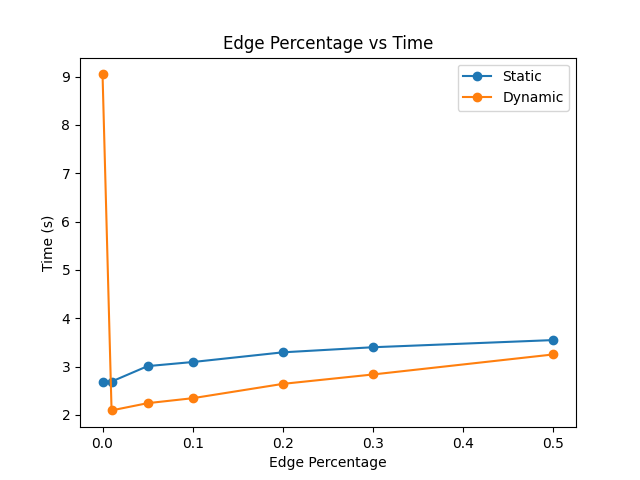
\includegraphics[width=\linewidth]{./Figures/Amazon0302.out.png}
        \caption{\texttt{Amazon0302}}
    \end{subfigure}
    \hfill
    \begin{subfigure}{0.3\textwidth}
        \centering
        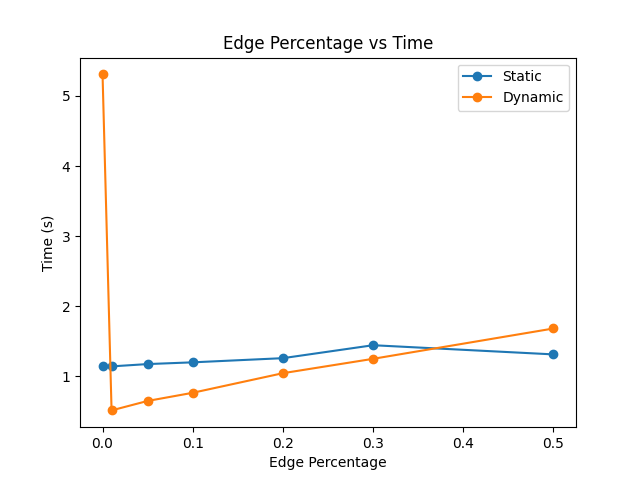
\includegraphics[width=\linewidth]{./Figures/Slashdot0902.out.png}
        \caption{\texttt{Slashdot0902}}
    \end{subfigure}
    \hfill
    \begin{subfigure}{0.3\textwidth}
        \centering
        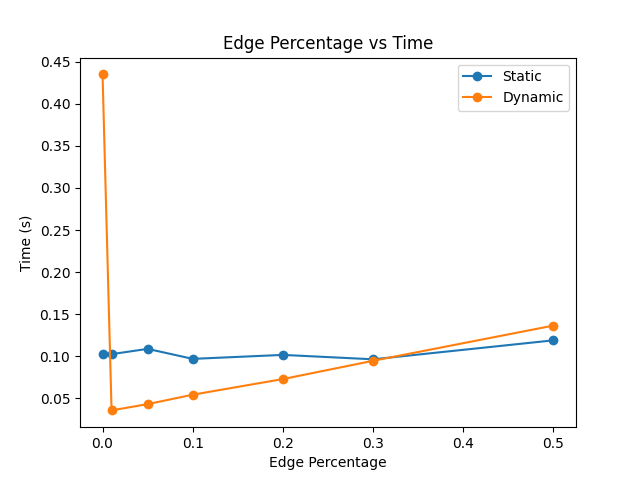
\includegraphics[width=\linewidth]{./Figures/Wiki-Vote.out.png}
        \caption{\texttt{Wiki-Vote}}
    \end{subfigure}
    \vspace{0.5cm}
    
    \begin{subfigure}{0.3\textwidth}
        \centering
        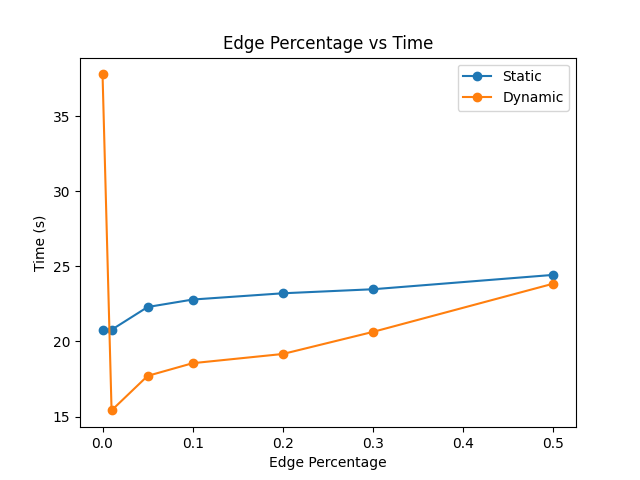
\includegraphics[width=\linewidth]{./Figures/WikiTalk.out.png}
        \caption{\texttt{WikiTalk}}
    \end{subfigure}
    \hfill
    \begin{subfigure}{0.3\textwidth}
        \centering
        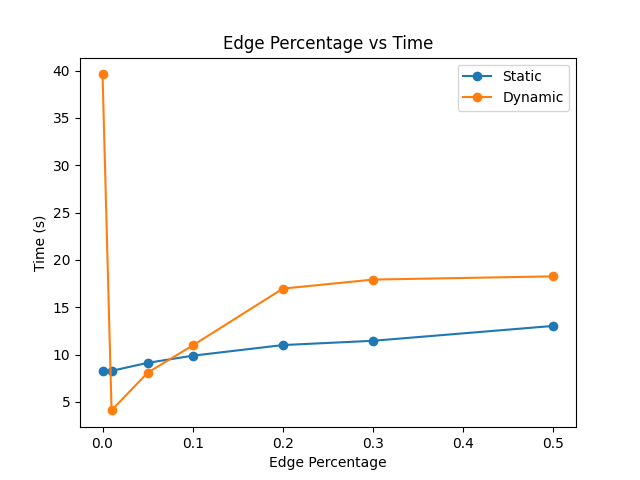
\includegraphics[width=\linewidth]{./Figures/web-BerkStan.out.png}
        \caption{\texttt{web-BerkStan}}
    \end{subfigure}
    \hfill
    \begin{subfigure}{0.3\textwidth}
        \centering
        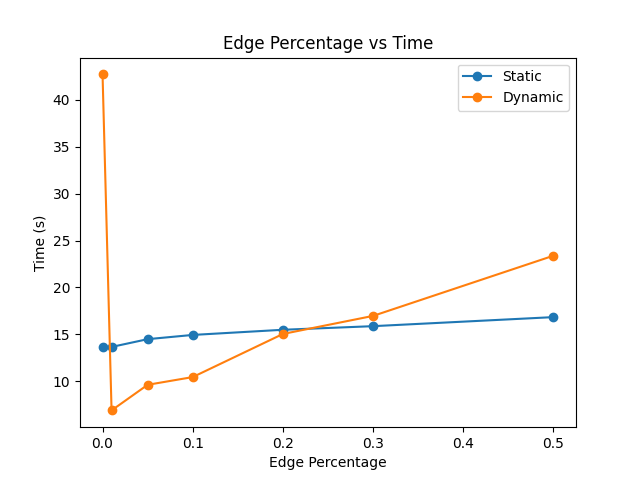
\includegraphics[width=\linewidth]{./Figures/web-Google.out.png}
        \caption{\texttt{web-Google}}
    \end{subfigure}
    \vspace{0.5cm}
    
    \begin{subfigure}{0.3\textwidth}
        \centering
        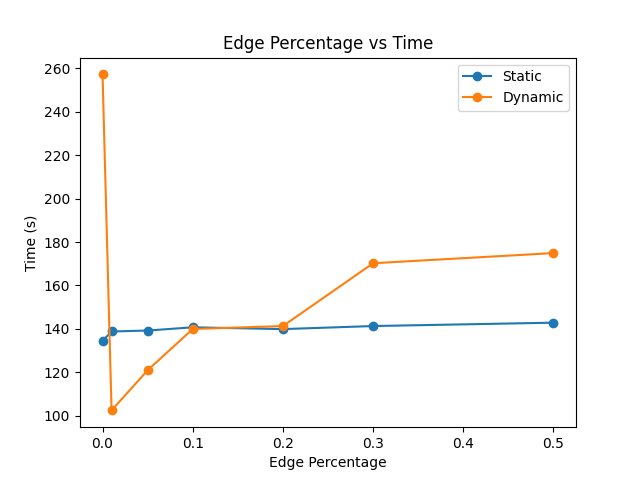
\includegraphics[width=\linewidth]{./Figures/big.png}
        \caption{\texttt{soc-pokec-relationships}}
    \end{subfigure}
    \hfill
    % Add more subfigures if needed
    \caption{Graphs Timings for \tableref{\ref{tab:graph_details}}}
    \label{fig:seven_images}
\end{figure}



